\newpage
\section{Implementierung}\label{sec:implementation}
Die App, die im Rahmen dieser Veranstaltung als Projekt entstanden ist, ist eine native Android App. Wir haben uns aufgrund der Vorkenntnisse dazu entschieden, die App nur für die Android Plattform zu entwickeln. Dazu haben wir die Entwicklungsumgebung Android Studio verwendet, die den Entwicklungsprozess von Android Apps stark vereinfacht. Als Programmiersprache wurde Kotlin verwendet, da diese mittlerweile zum Standard für die Entwicklung von Android Apps geworden ist. Außerdem haben wir uns dazu entschieden, die App mit dem Jetpack Compose UI Toolkit zu erstellen, da dieses ebenfalls den Standard für die Entwicklung von Benutzeroberflächen für die Android Plattform darstellt.

\subsection{App-Struktur}
Die Struktur der Anwendung besteht im Wesentlichen aus zwei Schichten: der Datenschicht und der Darstellungsschicht. Die Datenschicht stellt die Anwendungsdaten für die Benutzeroberfläche bereit, während die Darstellungsschicht für die Anzeige dieser Daten verantwortlich ist.

\medbreak

\begin{figure}[H]
    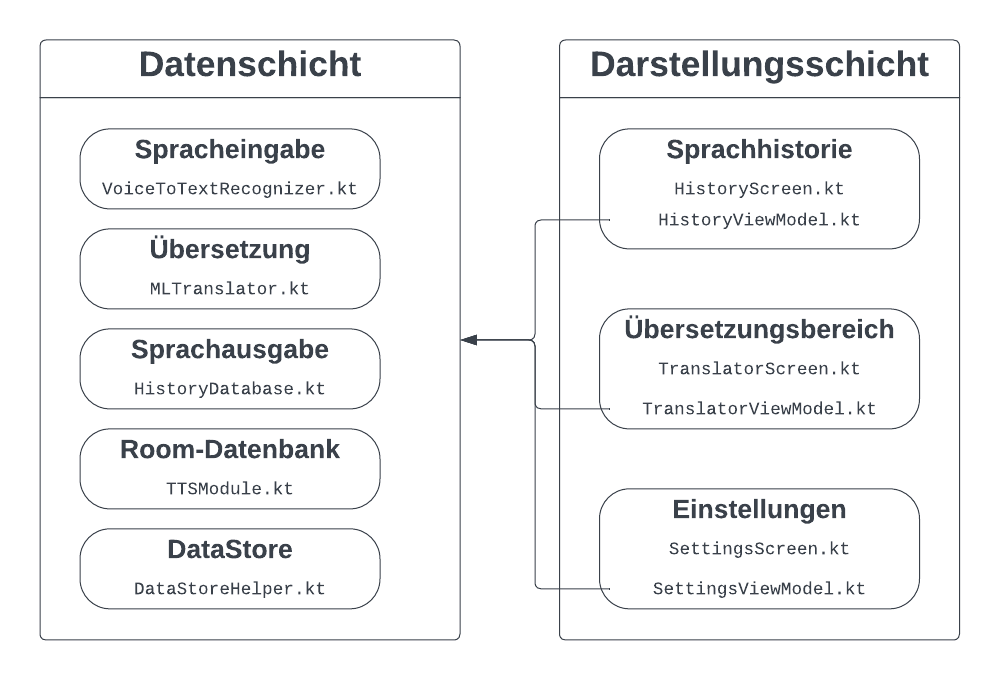
\includegraphics[width=\textwidth, center]{resources/SysAdmin_App_architecture.png}
    \caption[Diagramm: Aufbau der App]{Diagramm: Aufbau der App}
\end{figure}

Die Datenschicht besteht aus verschiedenen Modulen, von denen jedes eine bestimmte Aufgabe in der Anwendung ausführt. Diese Module sind über Dependency Injection in der gesamten Anwendung verfügbar und werden alle als Singleton-Objekte behandelt. Spezielle Module wurden für die Spracheingabe, die Übersetzung und die Sprachausgabe entwickelt, da diese die drei wichtigsten Komponenten der Anwendung darstellen. Zusätzlich gibt es ein Modul für den Zugriff auf die Room-Datenbank, welches eine SQL-Datenbank ist, in der die Sprachhistorie gespeichert wird. Außerdem gibt es ein Modul für den Zugriff auf den sogenannten \texttt{DataStore}, welcher eine lokale Schlüssel-Werte-Datenbank ist, in der die App-Einstellungen gespeichert werden. 

\bigbreak
\bigbreak

Die Darstellungsschicht ist in die einzelnen Bildschirme (Screens) der App unterteilt. Für jeden dieser Screens gibt es eine View, in der die Benutzeroberfläche mit Hilfe des UI-Toolkits Jetpack Compose erstellt wird. Jeder Screen besitzt auch ein zugehöriges Viewmodel, das als Schnittstelle zwischen der View und der Datenschicht fungiert. Die Daten werden über den sogenannten \texttt{UI-State} an den Screen übergeben. Dieser Datenaustausch wird durch die Verwendung von \texttt{Flows} realisiert, die einen Datenstrom zur Verfügung stellen, der auf Änderungen überwacht werden kann. Dadurch wird der Screen automatisch neu gerendert, sobald sich der \texttt{UI-State} ändert. Eine detailliertere Beschreibung dieser Screens erfolgt im nächsten Kapitel (Kapitel \ref{sec:implementation-ui}).

\subsection{Grafische Benutzeroberfläche}\label{sec:implementation-ui}
Unsere grafische Benutzeroberfläche ist in drei Bereiche unterteilt: die Sprachhistorie, in der die bisherigen Übersetzungen in einer Liste angezeigt werden; den Übersetzungsbereich, in dem Texte offline per Sprach- oder Tastatureingabe übersetzt und als Text oder Sprache ausgegeben werden können; und die Einstellungen, in denen Anpassungen an der Anwendung vorgenommen werden können. Die Navigation zwischen den drei Bereichen erfolgt über eine Schaltfläche am unteren Bildschirmrand.

\begin{figure}[H]
    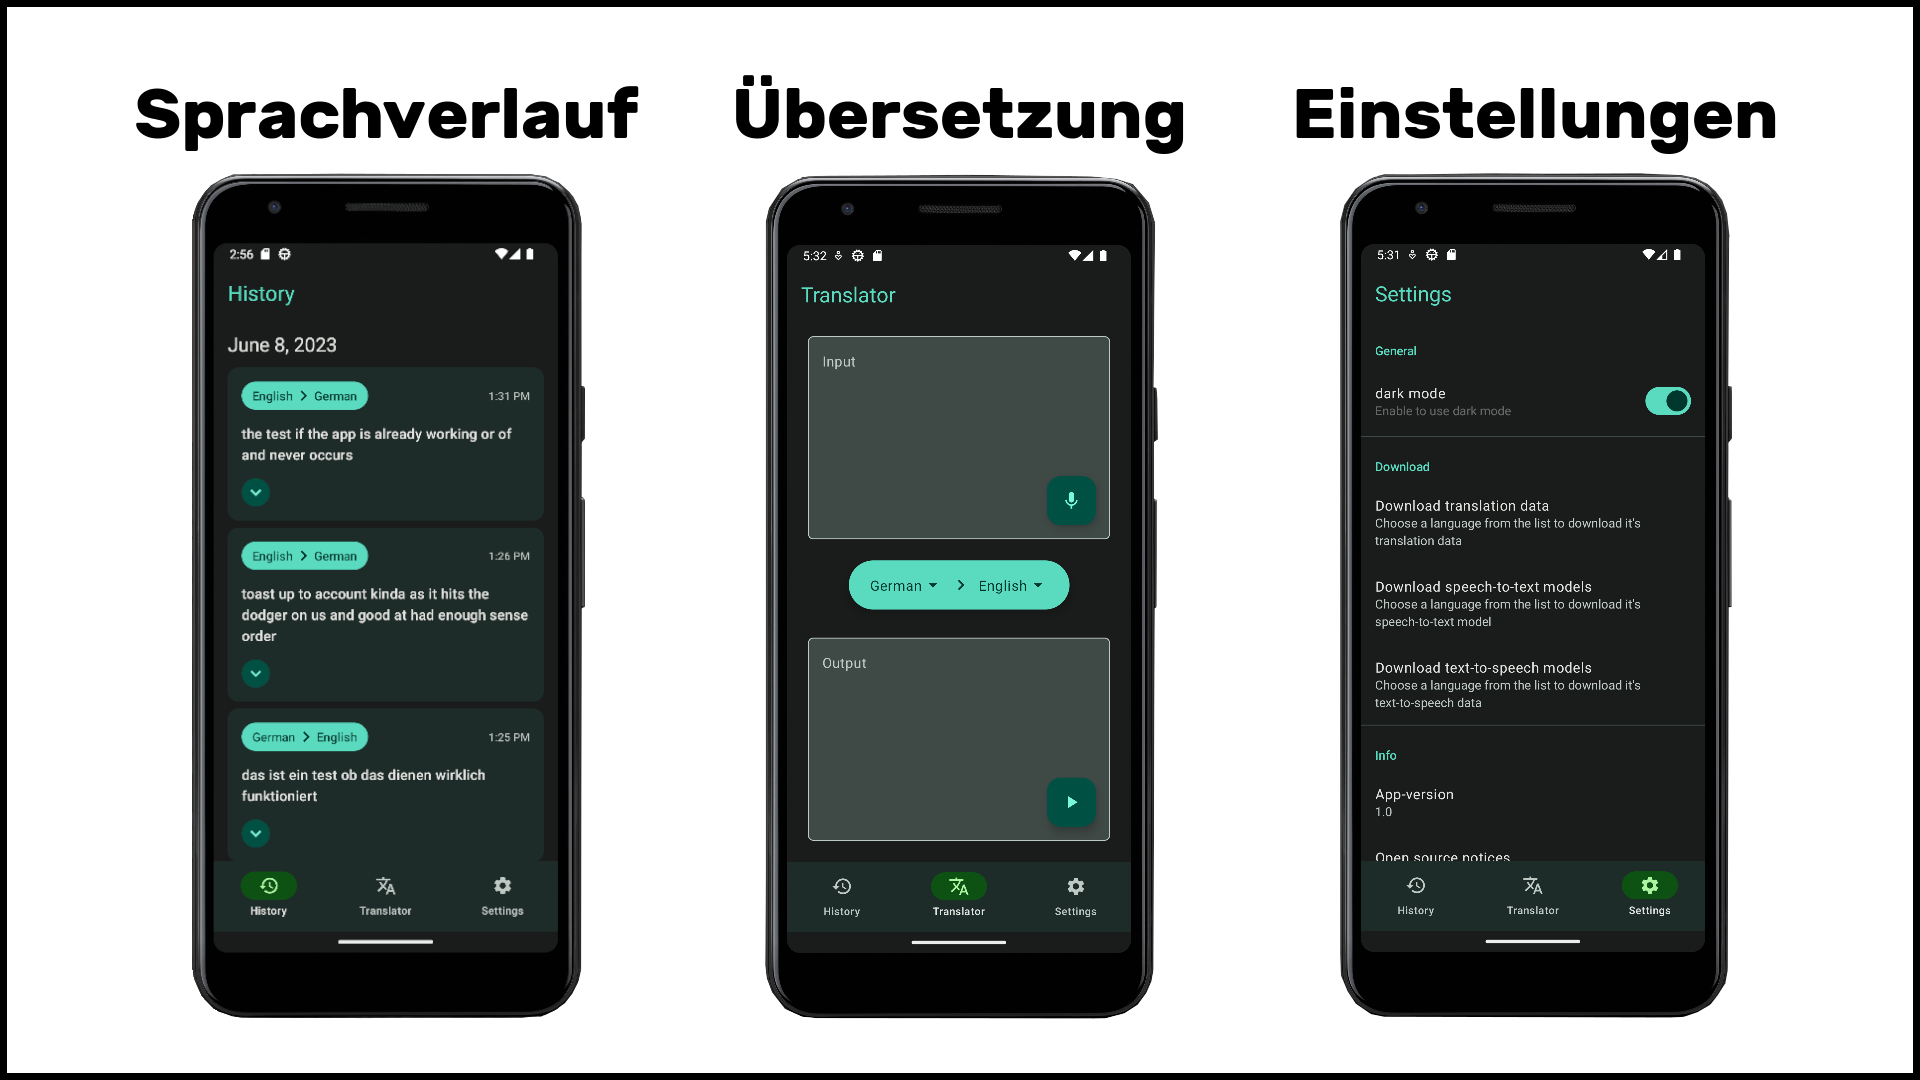
\includegraphics[scale=1, center]{resources/diagram_graphics_v02.png}
    \caption[Diagramm: Grafische Benutzeroberfläche]{Diagramm: Grafische Benutzeroberfläche}
\end{figure}

\subsubsection{Die Sprachhistorie}
Die Sprachhistorie bietet dem Benutzer die Möglichkeit, in der Vergangenheit durchgeführte Übersetzungen erneut einzusehen. Die Übersetzungen werden in einer übersichtlichen Liste angezeigt. Diese Liste ist nach dem Datum der letzten Übersetzung sortiert und nach dem Datum gruppiert.

Die Übersetzungen werden in einer Card angezeigt. Diese Card enthält zunächst Informationen über die verwendeten Sprachen, den eingegebenen Text und den Zeitpunkt der Übersetzung. Diese Cards können außerdem aufgeklappt werden, um die entsprechende Übersetzung anzuzeigen, und über eine Schaltfläche kann die Übersetzung aus der Sprachhistorie entfernt werden.

Die Daten der Sprachhistorie werden in der lokalen Room-Datenbank gespeichert. Für jede Übersetzung wird die Eingabesprache, die Ausgabesprache, der Eingabetext, der übersetzte Text, der Zeitstempel der Übersetzung und eine eindeutige ID gespeichert. Das Viewmodel der Sprachhistorie liest die Daten direkt aus der Room-Datenbank als \texttt{Flow}. Dadurch wird der \texttt{UI-State} automatisch geändert, sobald sich die Daten in der Datenbank ändern und die Benutzeroberfläche wird entsprechend neu gerendert.

\subsubsection{Der Übersetzungsbereich}
Der Übersetzungsbereich ist das Herzstück der Anwendung und stellt den zentralen Interaktionsbereich für den Benutzer dar. Hier hat der Benutzer die Möglichkeit, den gewünschten Text entweder manuell in das dafür vorgesehene Textfeld einzugeben oder per Spracheingabe zu sprechen. Für die Spracheingabe wird die Klasse \texttt{VoiceToTextRecognizer} verwendet, die es ermöglicht, gesprochenen Text in geschriebenen Text umzuwandeln.

Spricht der Benutzer in einer Sprache, für die kein entsprechendes Sprachpaket installiert ist, wird eine Fehlermeldung in Form einer Snackbar angezeigt. Nach Abschluss der Eingabe wird der eingegebene Text automatisch übersetzt und im zweiten Textfeld angezeigt. Die eigentliche Übersetzungsarbeit erfolgt durch direkte Kommunikation zwischen dem Viewmodel und der Klasse \texttt{MLTranslator}. Der eingegebene Text wird an den \texttt{MLTranslator} übergeben, der die Übersetzung durchführt und das Ergebnis asynchron zurückgibt.

Über einen Button im zweiten Textfeld kann sich der Benutzer den übersetzten Text per Sprachausgabe vorlesen lassen. Dazu wird das \texttt{TTSModule} verwendet, das die Funktion zur Ausgabe von Texten zur Verfügung stellt. Das Viewmodel ruft die entsprechende Funktion mit dem übersetzten Text auf, um die Sprachausgabe zu starten. Auch hier wird bei fehlenden Sprachpaketen eine Fehlermeldung ausgegeben, um den Benutzer zu informieren.

Zwischen den beiden Textfeldern für die Ein- und Ausgabe befindet sich eine Schaltfläche, mit der der Benutzer die Spracheinstellungen für die Ein- und Ausgabe festlegen kann. Es können nur die Sprachen ausgewählt werden, für die in den App-Einstellungen die entsprechenden Übersetzungspakete heruntergeladen wurden. Auf diese Weise wird sichergestellt, dass der Benutzer nur die verfügbaren Sprachen auswählen kann und eine reibungslose Übersetzung gewährleistet ist.

\subsubsection{Die Einstellungen}
Der letzte Bereich der App ist der Bereich der App-Einstellungen, der dem Benutzer verschiedene Optionen zur individuellen Anpassung der App bietet. Hier kann der Benutzer zwischen einem dunklen und einem hellen Erscheinungsbild der App wählen. Darüber hinaus besteht die Möglichkeit, die Sprachpakete für Spracheingabe, Übersetzung und Sprachausgabe herunterzuladen, um die App auch ohne aktive Internetverbindung nutzen zu können.

Für den Download der Sprachpakete für Spracheingabe und Übersetzung haben wir einen speziellen Bildschirm innerhalb der App implementiert. Dieser Bildschirm listet die zum Download verfügbaren Sprachen auf und ermöglicht es dem Benutzer, die gewünschten Pakete auszuwählen und herunterzuladen. Auf diese Weise kann der Benutzer gezielt die Sprachen auswählen, die er benötigt, und unnötigen Speicherplatzverbrauch vermeiden.

Für den Download von Sprachpaketen für die Sprachausgabe stellt Android einen eigenen Bildschirm zur Verfügung, der automatisch aufgerufen werden kann. Dieser Bildschirm übernimmt die Verwaltung der Pakete und ermöglicht es dem Benutzer, ohne weitere Implementierungsschritte die benötigten Sprachausgabepakete herunterzuladen.

Neben den Anpassungsoptionen und den Sprachpaketen enthält der Einstellungsbereich auch wichtige Informationen wie die aktuelle Version der App und Angaben zur Open-Source-Lizenz, die für eine Veröffentlichung der App notwendig sind.

\subsection{Spracheingabe}
Die Spracheingabe wurde zunächst über den Android SpeechRecognizer realisiert und später durch das Vosk-Projekt ersetzt. Grund dafür ist, dass die API des SpeechRecognizer zum Download von Sprachpaketen erst ab Android Version 13 zur Verfügung steht und somit nur für wenige Nutzer zugänglich ist.

Die erste Implementierung mit dem von Google entwickelten SpeechRecognizer war zunächst unproblematisch. Die entsprechende API ist gut dokumentiert, so dass die Transkriptionsfunktionalität sehr schnell implementiert werden konnte.

Die Implementierung der Vosk Spracherkennung warf nur wenige Probleme auf. In einem eigenen Modul wird das Paket initialisiert und dieses Modul bietet eine Schnittstelle, um den per Sprache eingegebenen Text zu transkribieren. Die einzigen Probleme, die mit Vosk auftraten, waren der Wechsel der Sprache und die Ausgabe des übersetzten Textes.

Beim Wechsel der Eingabesprache musste darauf geachtet werden, dass Vosk komplett neu initialisiert werden muss. Außerdem muss jedes Sprachmodell manuell heruntergeladen und integriert werden. Aus diesem Grund kann der Benutzer zwar die Sprachen für die Übersetzung herunterladen, nicht aber die Sprachen für die Eingabe. Dies führt zu einem erhöhten Speicherbedarf der Anwendung.

Bei der Ausgabe des aufgenommenen Textes tritt das Problem auf, dass Vosk nicht immer den endgültigen Text ausgibt. Man muss also zuerst nachfragen, ob es einen endgültigen Text gibt und wenn nicht, auf die letzte Version des Textes zurückgreifen.

\subsection{Übersetzung}
Die Übersetzungsfunktion unserer Anwendung basiert auf dem Google ML Kit Translator. Um den Google ML Kit Translator optimal nutzen zu können, haben wir eine eigene Klasse namens \texttt{MLTranslator} entwickelt, die zur Laufzeit als Singleton instanziiert wird. Diese Klasse ist über das Paket Dagger mittels Dependency Injection verfügbar. Die Klasse \texttt{MLTranslator} übernimmt die gesamte Übersetzungslogik mit dem ML Kit, so dass das Viewmodel lediglich die Funktion \texttt{startTranslate} aufrufen muss, um den übersetzten Text asynchron abzurufen.

Zusätzlich kann das Viewmodel die Quell- und Zielsprache an die Klasse \texttt{MLTranslator} übergeben, sobald der Benutzer diese ändert. Dies ermöglicht eine flexible Anpassung der Übersetzungssprachen zur Laufzeit. Durch diese Architektur wird das Viewmodel von der Komplexität der Übersetzungslogik entlastet und kann sich auf die Interaktion mit der Benutzerschnittstelle konzentrieren.

\subsection{Sprachausgabe}
Die Sprachausgabe auf Basis von Android \texttt{TextToSpeech} haben wir ebenfalls in einer eigenen Klasse namens \texttt{TTSModule} entwickelt. Auch diese Klasse wird zur Laufzeit als Singleton-Objekt instanziiert und steht ebenfalls über die Dependency Injection zur Verfügung.

Die Klasse \texttt{TTSModule} übernimmt die komplette Initialisierung der Android-Funktion \texttt{TextToSpeech}. Somit muss das Viewmodel nur noch die Funktion \texttt{speak} aufrufen. Dieser wird der Text als String und die Sprache als \texttt{Locale} übergeben. Damit wird der übergebene Text in die entsprechende Sprache synthetisiert und über die Lautsprecher des Gerätes ausgegeben. Ist die übergebene Sprache nicht verfügbar, wird ein Fehler ausgegeben.